\documentclass[14pt]{extarticle}
\usepackage[english,ukrainian]{babel}
\usepackage[utf8]{inputenc}
\usepackage{amsmath,amssymb}
\usepackage{parskip}
\usepackage{graphicx}
\usepackage{tcolorbox}
\tcbuselibrary{skins}
\usepackage[framemethod=tikz]{mdframed}
\usepackage{chngcntr}
\usepackage{enumitem}
\usepackage{float}
\usepackage{subfig}
\usepackage{esint}
\usepackage[top=2.5cm, left=3cm, right=3cm, bottom=4.0cm]{geometry}
\usepackage[table]{xcolor}
\usepackage{algorithm}
\usepackage{algpseudocode}
\usepackage{listings}
\usepackage{dsfont}

% Chad's colors:
% See http://web.njit.edu/~kevin/rgb.txt.html for possibilities
\definecolor{ChadDarkBlue}{rgb}{.1,0,.2}  
\definecolor{ChadBlue}{rgb}{.1,.1,.5}  
\definecolor{ChadRoyal}{rgb}{.2,.2,.8}  
%\definecolor{ChadGreen}{rgb}{0,.35,.1}
%\definecolor{ChadGreen}{rgb}{0,.5,.25}  % Too bright
%\definecolor{ChadGreen}{rgb}{0,.4,.2}    % Still too bright
\definecolor{ChadGreen}{rgb}{0,.4,0}    % Dark Green
%\definecolor{ChadRed}{rgb}{.8,.1,.2}    % Too bright
\definecolor{ChadRed}{rgb}{.5,0,.5}  % purple

%%% HYPERLINKS %%%%%%%%%%%%%%%%%%%%%
\usepackage[colorlinks,breaklinks,   % deleted ps2pdf 11/6/15
     bookmarks=false,
     pdfstartview=Fit,  % for fitting entire page; FitW just fits width
     pdfview=Fit,       % after traversing a hyperlink
     linkcolor=ChadRed,
     urlcolor=ChadRed,
     citecolor=ChadGreen,
     hyperfootnotes=false
         ]{hyperref}
\usepackage[figure,table]{hypcap} % Correct a problem with hyperref
\urlstyle{rm} % so it doesn't use a typewriter font for url's.
\usepackage[nameinlink]{cleveref}

\title{Домашня робота \#2 з курсу ``Моделювання на \textit{Python}''}
\author{Студента 3 курсу групи МП-31 Захарова Дмитра}
\date{\today}

\begin{document}

\maketitle

\section*{Умова}

Розглядається задача випадкового блукання: нехай ми стоїмо у точці $x=0$ і на кожному кроці з ймовірністю $\frac{1}{2}$ рухаємось праворуч, а з ймовірністю $\frac{1}{2}$ -- ліворуч. Завдання, дослідити:
\begin{itemize}
    \item Частку кроків, коли $x$ координата додатня.
    \item Кількість змін знаку $x$ координати.
\end{itemize}

\begin{figure}
    \centering
    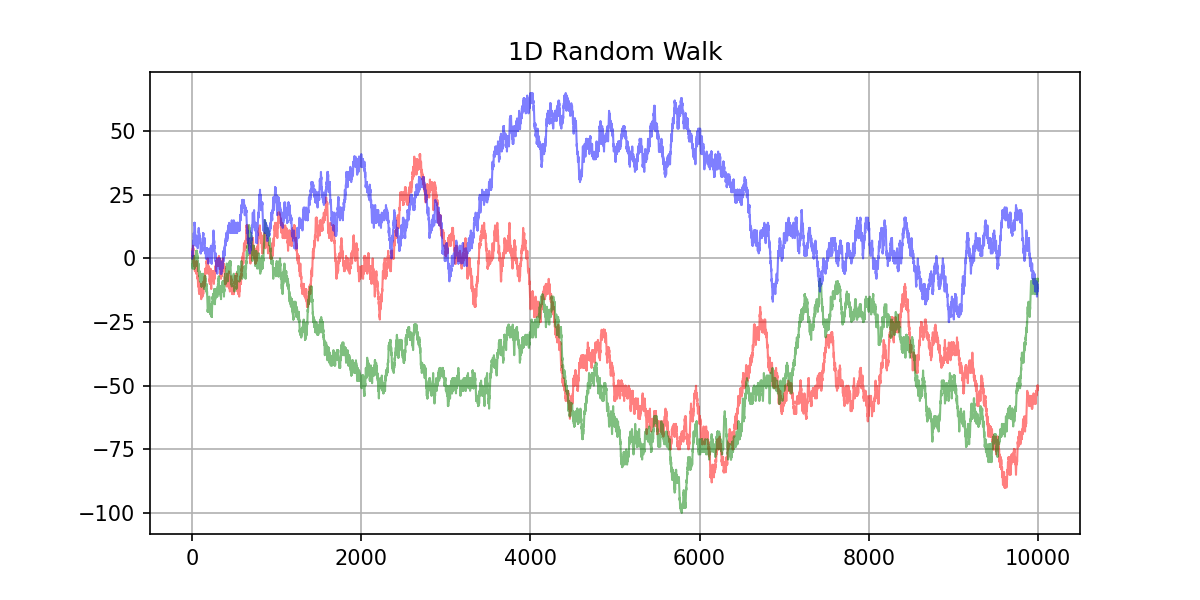
\includegraphics[width=0.7\textwidth]{images/hw_2/random_walk.png}
    \caption{Процес випадкового блукання}
    \label{fig:preview}
\end{figure}

\section{Частка кроків з додатною координатою}

\textbf{Умова.} Проведіть експеримент для знаходження часу, коли координата є додатною. Що вони означають у термінах випадкових шляхів? Спробуйте розділити відрізок $[0,1]$ на $20,30$ частин. Що можна сказати тепер?

\textbf{Відповідь.} Трошки формалізуємо постановку задачі. Нехай $X_i$ -- випадкова величина, що позначає $x$ координату на $i^{\text{ому}}$ кроці (при цьому вважаємо, що $X_0=0$). 

Якщо випадкове блукання відбувається за $N$ кроків, то по суті ми маємо набір випадкових величин $\{X_i\}_{i=0}^N$.

Коли ми знаходимо середню частку перебування на додатній координаті, то ми знаходимо наступну випадкову величину:
\begin{equation}
    \nu_N := \frac{1}{N}\sum_{i=0}^N \mathds{1}[X_i \geq 0].
\end{equation}
Ця величина розподілена по деякому закону, тобто існують значення:
\begin{equation}
    \mathbb{P}\left(\nu_N = \frac{1}{n}\right), \; n \in \{1,\dots,N\}
\end{equation}
Гістограма, що ми будуємо, по суті і є наближеним розподілом. Тобто, нехай ми проводимо $m$ експериментів, на кожному робимо $N$ кроків, а далі на основі цих $m$ експериментів ми ділимо відрізок на $k$ частин і будуємо гістограму. 

Нехай ми отримали набір значень $\{f_i\}_{i=0}^{k-1}$, де $f_i$ -- частота знаходження на додатній $x$ координаті від $\frac{i}{k}$ до $\frac{i+1}{k}$ частку кроків. Гіпотеза наступна: 
\begin{equation}
    \lim_{m \to \infty} f_i = \mathbb{P}\left(\frac{i}{k} \leq \nu_N \leq \frac{i+1}{k}\right), \; i \in \{0,\dots,k-1\},
\end{equation}
тобто якщо  зробити нескінченно багато експериментів, то $f_i$ мають давати приблизний розподіл $\mathbb{P}\left(\nu_N = \frac{1}{n}\right)$.

\begin{figure}
    \centering
    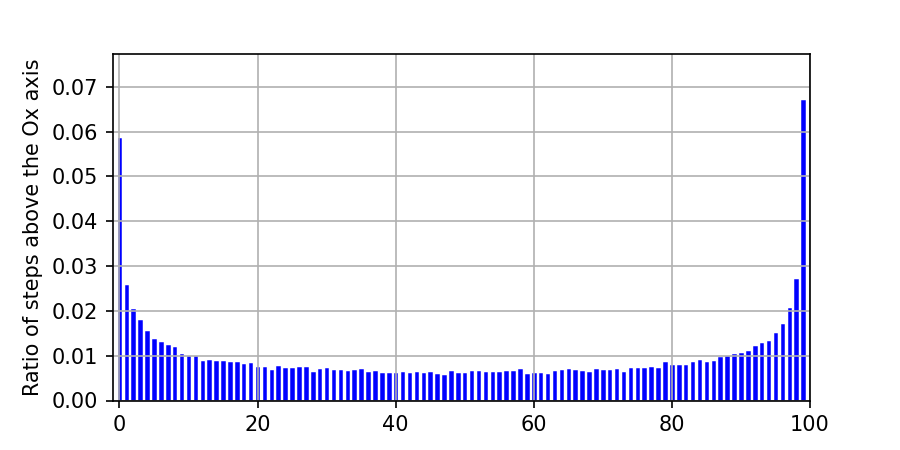
\includegraphics[width=\textwidth]{images/hw_2/positive_y_experiment.png}
    \caption{Гістограма розподілу частоти знаходження на додатній координаті}
    \label{fig:histogram_1}
\end{figure}

Якщо провести експеримент для $N=10000,k=100,m=10000$, то отримаємо графік, що зображено на рис. \ref{fig:histogram_1}. Можна побачити цікаву особливість -- майже уся густина розподілу знаходиться по краях малюнку. Тобто, або майже увесь час або ми знаходимось на додатній координаті, або весь час на від'ємній.

Звідси, можна сформулювати наступну гіпотезу:

\textbf{Гіпотеза 1.} Гранично, розподіл $\nu_N$ записується так:
\begin{equation}
    \lim_{N \to \infty}\mathbb{P}\left(\nu_N = \frac{1}{n}\right) = \begin{cases}
        \frac{1}{2}, & n = 1 \\
        \frac{1}{2}, & n = N \\
        0, & n \neq 1 \wedge n \neq N
    \end{cases}
\end{equation}
Це було б достатньо логічно, бо в такому разі математичне сподівання:
\begin{equation}
    \mathbb{E}[\nu_N] \xrightarrow[N \to \infty]{} \mathbb{P}(\nu_N = 1) + \mathbb{P}\left(\nu_N = \frac{1}{N}\right) \times \frac{1}{N} \xrightarrow[N \to \infty]{} \frac{1}{2}, 
\end{equation}
тобто ми приблизно половину часу знаходимось на додатній координаті.

\section{Частка змін лідерства}

Тепер розглянемо задачу, де ми шукаємо частоту події ``зміна знаку координати''. 

Нехай після експерименту на $N$ кроках ми отримали набір $x$ координат $\{x_i\}_{i=0}^N$. Тоді, будемо вважати, що на $j^{\text{ому}}$ кроці відбувалась зміна лідерства якщо:
\begin{equation}
    x_j = 0 \wedge x_{j-1}x_{j+1} < 0, \; \text{для} \; j \in \{1,\dots,N-1\}.
\end{equation}
Тобто, на $j^{\text{ому}}$ кроці ми повернулись у початок координат, а на $(j+1)^{\text{ому}}$ кроці ми змінили знак відносно $(j-1)^{\text{ого}}$ кроку. Формально, введемо набір випадкових величин $\{Y_j\}_{j=1}^{N-1}$, де
\begin{equation}
    Y_j := \mathds{1}\left[X_j=0 \wedge X_{j-1}X_{j+1} < 0\right]
\end{equation}
і будемо розглядати $\xi_N := \frac{1}{N-1}\sum_{j=1}^{N-1}Y_j$. Якщо побудувати гістограму для $\xi_N$ на відрізку $[0.0,0.1]$, то отримаємо результат на рис. \ref{fig:histogram_2}.
\begin{figure}
    \centering
    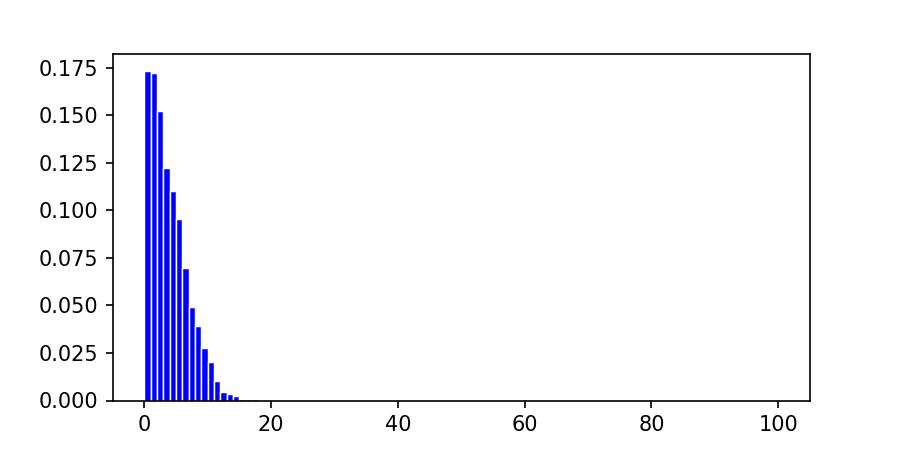
\includegraphics[width=\textwidth]{images/hw_2/switches_number_experiment.png}
    \caption{Гістограма розподілу частоти зміни знаку координати для відрізку $[0.0,0.1]$.}
    \label{fig:histogram_2}
\end{figure}

Тут вже видна наступна особливість: майже завжди в експерименті $\hat{\xi}_N < 0.02$, тобто густина майже повністю знаходиться біля $0$. Також, якщо знайти середнє значення усіх відношень кількостей змін лідерства до $N$, то вийде значення доволі близьке до $0$. Звідси, можна сформулювати наступні дві гіпотези:

\textbf{Гіпотеза 2.} Гранично,
\begin{equation}
    \lim_{N \to \infty}\mathbb{P}[\xi_N=\alpha] = \mathds{1}[\alpha=0].
\end{equation}

\textbf{Гіпотеза 3.} $\lim_{N \to \infty}\mathbb{E}[\xi_N] = 0$.

\end{document}

